\documentclass{beamer}
\usepackage{amsmath,amssymb,amsthm,slashed, euscript}
\usepackage{mathrsfs} 

\usepackage{tikz}
\usepackage{tikz-cd}
\usetikzlibrary{cd}

\textwidth=110mm


\title{Algebraic topology of $C^*$-algebras}
\institute
{
Algebreas in analisys\\
https://arxiv.org/abs/2511.09189
}

\author{Petr R. Ivankov  }



\theoremstyle{plain}
\newtheorem{defn}{Definition}
\newtheorem{rem}{Remark}
\newtheorem{exm}{Example}
\newtheorem*{claim}{Claim}
\newtheorem{prop}{Proposition}
\newtheorem{empt}[prop]{}%[section]
\newtheorem{lem}{Lemma}%[section]
\newtheorem{thm}{Theorem}%[section]

\newcommand{\Dl}{\Delta}
\newcommand{\Z}{\mathbb{Z}}
\newcommand{\A}{\mathcal{A}}
\newcommand{\be}{\begin{equation}}
\newcommand{\ee}{\end{equation}}
	\newcommand{\bean}{\begin{eqnarray*}}
	\newcommand{\eean}{\end{eqnarray*}}
\newcommand{\Ga}{\Gamma}
\newcommand{\B}{\mathcal{B}}
\newcommand{\Cc}{\mathcal{C}}
\newcommand{\C}{\mathbb{C}}
\newcommand{\R}{\mathbb{R}}
\newcommand{\D}{\mathcal{D}}
\newcommand{\G}{\mathcal{G}}
\newcommand{\Hc}{\mathcal{H}}
\newcommand{\Lc}{\mathcal{L}}
\newcommand{\Pc}{\mathcal{P}}
\newcommand{\Sc}{\mathcal{S}}
\newcommand{\U}{\mathcal{U}}
\newcommand{\rar}{\rightarrow}
\newcommand{\Ef}{\mathbb{E}}
\newcommand{\desc}{\mathfrak{desc}}
\newcommand{\rep}{\mathfrak{rep}}
\newcommand{\eps}{\varepsilon}
\newcommand{\T}{\mathbb{T}}


%Uppercase Gothic characters
\newcommand{\gtA}{\mathfrak{A}}
\newcommand{\gtB}{\mathfrak{B}}
\newcommand{\gtM}{\mathfrak{M}}
\newcommand{\gtN}{\mathfrak{N}}
\newcommand{\gtP}{\mathfrak{P}}
\newcommand{\gtS}{\mathfrak{S}}

%Lowercase Gothic characters
\newcommand{\gtf}{\mathfrak{f}}
\newcommand{\gtg}{\mathfrak{g}}

%Bold Characters
\newcommand{\Cb}{\mathbb{C}}
\newcommand{\Nb}{\mathbb{N}}
\newcommand{\Rb}{\mathbb{R}}
\newcommand{\Zb}{\mathbb{Z}}

%Uppercase Greek characters
\newcommand{\Gm}{\Gamma}
\newcommand{\Te}{\Theta}
\newcommand{\Om}{\Omega}
\newcommand{\s}{ }

%Lowercase Greek characters
\newcommand{\al}{\alpha}
\newcommand{\gm}{\gamma}
\newcommand{\dl}{\delta}
\newcommand{\sg}{\sigma}
\newcommand{\ph}{\varphi}
\newcommand{\te}{\theta}
\newcommand{\ze}{\zeta}
\newcommand{\lift}{\mathfrak{lift}}

\newcommand{\Id}{\mathrm{Id}}
\newcommand{\Aut}{\mathrm{Aut}}
\newcommand{\Coo}{{\mathrm{C}}^\infty}
\newcommand{\alg}{\mathrm{alg}}
\newcommand{\diag}{\mathrm{diag}}
\newcommand{\spinc}{\textbf{$spin^c$}}
\newcommand{\Hom}{\mathrm{Hom}}
\newcommand{\supp}{\mathrm{supp}}
\newcommand{\codim}{\mathrm{codim}}
\newcommand{\Ccl}{\mathbf{C}l}
\newcommand{\xto}{\xrightarrow}

\newcommand{\lto}{\longrightarrow}
\newcommand{\ox}{\otimes}
\newcommand{\nb}{\nabla}
\newcommand{\sS}{\mathcal{S}}
\newcommand{\Dn}{D\!\!\!\!/}
%\newcommand{\ij}{{i,j}}
\newcommand{\aC}{\ensuremath{\underline{\Cb}} }
\newcommand{\scp}[2]{\left\langle{#1},{#2}\right\rangle}
\newcommand{\op}[1]{J{#1}J^\dag}
\newcommand{\K}{\mathcal{K}} 
\newcommand{\F}{\mathcal{F}} 
\newcommand{\E}{\mathcal{E}} 
\newcommand{\sA}{\mathcal{A}} 
\newcommand{\sB}{\mathcal{B}}       %%
\newcommand{\sC}{\mathcal{C}}       %%
\newcommand{\sD}{\mathcal{D}}       %%
\newcommand{\sE}{\mathcal{E}}       %%
\newcommand{\sF}{\mathcal{F}}       %%
\newcommand{\sG}{\mathcal{G}}       %%
\newcommand{\sH}{\mathcal{H}}       %%
\newcommand{\sI}{\mathcal{I}}       %%
\newcommand{\sJ}{\mathcal{J}}       %%
\newcommand{\sK}{\mathcal{K}}       %%
\newcommand{\sL}{\mathcal{L}}       %%
\newcommand{\sM}{\mathcal{M}}       %%
\newcommand{\sN}{\mathcal{N}}       %%
\newcommand{\sO}{\mathcal{O}}       %%
\newcommand{\sP}{\mathcal{P}}       %%
\newcommand{\sQ}{\mathcal{Q}}       %%
\newcommand{\sR}{\mathcal{R}}       %%
\newcommand{\sT}{\mathcal{T}}       %%
\newcommand{\sU}{\mathcal{U}}       %%
\newcommand{\sV}{\mathcal{V}}       %%
\newcommand{\sX}{\mathcal{X}}       %%
\newcommand{\sY}{\mathcal{Y}}       %%
\newcommand{\sZ}{\mathcal{Z}}       %%
\newcommand{\N}{\mathbb{N}}                  %% 
\newcommand{\rank}{\mathrm{rank}}                  %% 

\renewcommand{\a}{\alpha}     
\newcommand{\la}{\lambda}     
\newcommand{\La}{\Lambda}
\newcommand{\bt}{\beta}           %% short for  \beta
\DeclareMathSymbol{\onto}{\mathrel}{AMSa}{"10}
 
    
\newcommand{\bydef}{\stackrel{\mathrm{def}}{=}}  
\newcommand{\hookto}{\hookrightarrow}        %% abbreviation
  
\begin{document}

\begin{frame}
  \titlepage
\end{frame}

\begin{frame}
Development of the (co)homology theory of $C^*$-algebras such that: 
\begin{itemize}
	\item for any commutative $C^*$-algebra $C\left(\sX \right)$ it coincides with  (co)homology theory of $\sX$.
	\item the theory is not trivial even for algebras having one-point  spectrum.
\end{itemize}
\end{frame}
\begin{frame}
	\begin{thm}\label{gelfand-naimark_I_thm} (Commutative Gelfand-Na\u{\i}mark theorem). 
		Let $A$ be a commutative $C^*$-algebra and let $\mathcal{X}$ be the spectrum of A. There is the natural $*$-isomorphism $\gamma:A \xrightarrow{\cong} C_0(\mathcal{X})$.
	\end{thm}
	\begin{lemma}\label{lem_g_i_lem} (\alert{ Ivankov}) (Generalized commutative Gelfand theorem).
		If $\sX$ is a locally compact, Hausdorff space then  is a natural  homeomorphism $ \mathfrak{Gelfand}_\sX: \mathfrak{Gelfand}\left(C_0\left( \sX\right)  \right)\cong \sX$.
	\end{lemma}
		\begin{lemma} (\alert{ Ivankov}) Let $A$ be a $C^*$-algebra which is represented by locally trivial bundle $\E\onto \sX$ such that
			\begin{itemize}
				\item $\sX$ is the Hausdorff spectrum of $A$,
				\item any fiber of $\E$ is a $C^*$-algebra of compact operators $\K = \K\left(\sH \right)$. 
			\end{itemize}
			Then $A$ uniquely depends on the Gelfand space of $A$.
	\end{lemma}
	
	
	
\end{frame}
\section{Introduction}

%\begin{frame}
	
%	\begin{figure}
%		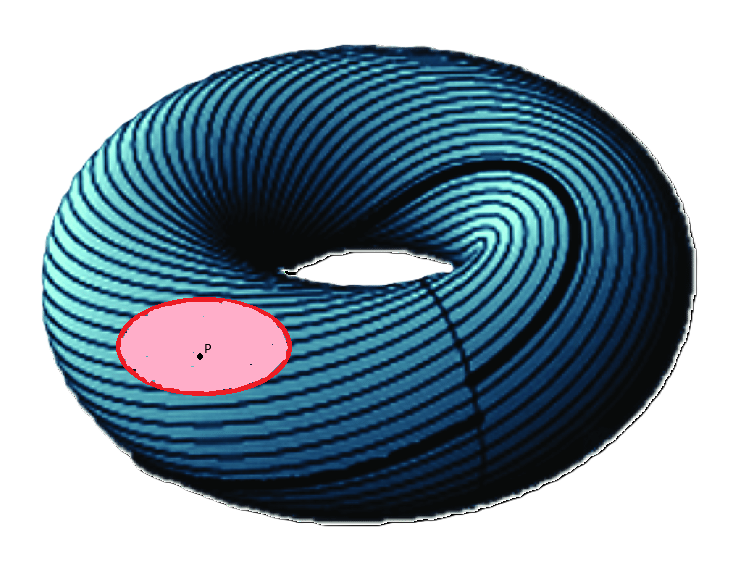
\includegraphics[width=\linewidth]{PICTURE.png}
%		\caption{A boat.}
%		\label{fig:boat1}
%	\end{figure}
%Irrational rotation $C^*$-algebra $C^*_r\left( M, \mathcal F\right)$ and its one-sided ideal.
%end{frame}
\begin{frame}
		\begin{definition}\label{upper_defn}
	Let $A$ be a partially ordered set, $S$ a subset of $A$. We say an element $a \in A$
	is a \alert{ meet} (or \alert{ greatest lower bound}) for $S$, and write $a = \wedge S$, if 
	\begin{enumerate}
		\item [(a)] $a$ is an lower bound for $S$, i.e. $a \le s$ for all $s \in S$, and 
		\item [(b)] if $b$ satisfies $\forall \in S\quad  b \le s$, then $b \le a$. 
	\end{enumerate}
	The antisymmetry axiom  ensures that the join of $S$, if it exists, is 
	unique. If $S$ is a two-element set $\{s, t\}$, we write $s \wedge t$ for $\wedge \{s, t\}$ and if $S$	is the empty set $\emptyset$, we write $0$ for  $\wedge \emptyset$.
\end{definition}

\begin{definition}\label{lattice_defn}
	A \alert{meet-semilattice} is a partially ordered set which supports for any finite set the  greatest lower bound.
\end{definition}
\begin{definition}\label{filter_defn}
	A subset $\mathfrak F$ of a meet-semilattice $A$ is said to be an \alert{ filter} if
	\begin{enumerate}
		\item [(a)] $\mathfrak F$ is a sub-meet-semilattice of $A$; i.e. $1\in A$, and $a, b \in \mathfrak F$  imply  	$a \wedge b \in \mathfrak F$; and
		\item [(b)] $\mathfrak F$ is a lower set; i.e. $a \in \mathfrak F$ and $ a\le b$ imply $b \in \mathfrak F$.  
	\end{enumerate}
\end{definition}
\end{frame}
\section{Gelfand space}
\begin{frame}
		Any homomorphism $\phi : L' \to L''$ of {semi}-{lattices} yields a map
		of filers
		\be\label{filtermap_eqn}
		\left\{I_\la\right\}_{\la \in \La}	\mapsto \text{ minimal filter containing } \left\{\phi\left( I_\la\right) \right\}_{\la \in \La}
		\ee
\begin{definition}\label{ultra_filter_defn}
	A maximal filter is an \alert{ultrafilter}.
\end{definition}		
		\begin{example}\label{space_semi_exm}
			If $\sX$ is a topological space then the $\sX$-\alert{semi}-\alert{lattice} is  a  meet-semilattice $\mathfrak{Lattice}\left( \sX\right)$ such that elements of $\mathfrak{Lattice}\left( \sX\right)$ are open subsets of $\sX$ and one has
			\be\label{x_lat_eqn}
			\begin{split}
				\sU' \wedge \sU''\bydef \sU' \cap \sU'',\\
				\sU' \le \sU'' \quad \Leftrightarrow\quad \sU'' \subset \sU',\\
				0 \bydef \emptyset.
			\end{split}
			\ee
			A set of neighborhoods of a point of Hausdorff space is an ultrafilter.
		\end{example}
	\label{ultra_filter_rem}
			From the Zorn’s lemma it follows that any filter is a subset of an	ultrafilter.

		
	\end{frame}

	\begin{frame}
\begin{definition}\label{lattice_a_defn}
	If $A$ be a $C^*$-algebra then $A$-\alert{semi}-\alert{lattice} is a meet-semilattice of closed left ideals such that 
	\be\label{meet_eqn}
	\begin{split}
		L' \wedge L''\bydef L' \cap L'',\\
		L' \le L'' \quad \Leftrightarrow\quad L' \subset L'',\\
		0 \bydef \{0\}\subset A
	\end{split}
	\ee
	We denote this semilattice by $\mathfrak{Lattice}\left( A\right)$ and denote by $\mathfrak{Filters}\left( A\right)$  a set of filers.
\end{definition}
\begin{definition}\label{ultrafilters_space_defn}
	If $\mathfrak{Ultrafilters}\left(A \right)$ is a set of ultrafilters of the meet-semilattice $\mathfrak{Lattice}\left( A\right)$ then for any closed left ideal $L \subset A$ denote by
	$$
	\mathfrak{Ultrafilters}\left(A \right)_L	\bydef \left\{\left. x \in \mathfrak{Ultrafilters}\left(A \right) \right| \exists L' \in x\quad L'\cap L = \{0\} \right\}
	$$
	The \alert{space of} $A$-\alert{ultrafilters} is a set $\mathfrak{Ultrafilters}\left(A \right)$ with a  the smallest topology o such that all sets $\mathfrak{Ultrafilters}\left(A \right)_L$ are open.
	
\end{definition}
\end{frame}
\begin{frame}

\begin{rem}
If $A = C_0\left( \sX\right)$ then $\mathfrak{Lattice}\left( A\right)\cong \mathfrak{Lattice}\left(\sX\right)$, $\mathfrak{Filters}\left( A\right)\cong \mathfrak{Filters}\left(\sX\right)$ and $\mathfrak{Ultrafilters}\left( A\right)\cong \mathfrak{Ultrafilters}\left(\sX\right)$.
\end{rem}
\begin{thm}
	One has:
	\begin{enumerate}
		\item [(a)] 	A topological space $\sX$ is Hausdorff if and only if every ultrafilter on $\sX$ has at most one limit.
		\item[(b)]   	A topological space $\sX$ is compact if and only if every ultrafilter has at least one limit.
	\end{enumerate} 
\end{thm}	
\begin{rem}
	If $\sX$ is locally compact then there are "infinite ultrafilters" which do not correspond to points of $\sX$.
\end{rem}
\end{frame}
\begin{frame}
Here we would like exclude "infinite ultrafilters".
	\begin{thm}\label{pedersen_ideal_thm}  
	% THEOREM 5.6.1
	For each $C^*$-algebra $A$ there is a dense hereditary ideal $K(A)$,
	which is minimal among dense ideals.
	\end{thm}
\begin{definition}\label{pedersen_ideal_defn}
	The ideal $K\left( A\right) $  is said to be the \alert{ Pedersen's ideal of $A$}. %Henceforth Pedersen's ideal shall be denoted by $K(A)$.
	\end{definition}
	One has $K\left( C_0\left( \sX\right) \right) = C_c\left(\sX \right)$ 
	\begin{definition}\label{gelfand_space_defn}(\alert{ Ivankov})
		An ultrafilter  $x \in \mathfrak{Ultrafilters}\left(A \right)$ is a \alert{finite point} if there is a nontrivial element $a\in K\left( A\right)\setminus\{0\}$ such that 
		$$
		Aa \in x.
		$$
		The \alert{Gelfand space} $\mathfrak{Gelfand}\left(A \right)$ of $C^*$-algebra $A$ is a topological subspace  of the {space of} $A$-{ultrafilters} (cf. Definition \ref{ultrafilters_space_defn})
		$$
		\mathfrak{Gelfand}\left(A \right)\bydef \left\{\left. x \in \mathfrak{Ultrafilters}\left(A \right)\right| \exists L \in x \quad L \text{ is a finite point}\right\}.
		$$
	\end{definition}
	
\end{frame}
\begin{frame}
	\begin{thm}\label{gelfand-naimark_thm} (Commutative Gelfand-Na\u{\i}mark theorem). 
		Let $A$ be a commutative $C^*$-algebra and let $\mathcal{X}$ be the spectrum of A. There is the natural $*$-isomorphism $\gamma:A \xrightarrow{\cong} C_0(\mathcal{X})$.
	\end{thm}
\begin{lemma}\label{lem_g_lem} (\alert{ Ivankov}) (Generalized commutative Gelfand theorem).
	If $\sX$ is a locally compact, Hausdorff space then  is a natural  homeomorphism $ \mathfrak{Gelfand}_\sX: \mathfrak{Gelfand}\left(C_0\left( \sX\right)  \right)\cong \sX$.
	\end{lemma}
	
\end{frame}
\begin{frame}
\begin{definition}\label{belongs_defn}
	Let $A$ be a $C^*$ -algebra and let $\hat A$ be the spectrum of $A$. An element $\xi \in \mathfrak{Gelfand}\left(A \right)$  \alert{belongs to} $x \in \hat A$ if one has
	\bean\label{belongs_eqn}
	\forall L \in \xi \quad \rep_x\left(L\right) \neq \{0\} 
	\eean
	where $\rep_x : A \to B\left(\sH_x \right)$ is an irreducible representation.
	
\end{definition}

	Under the hypothesis of the above Definition   if $x', x'' \in \hat A$ with $x' \neq x''$ and $\xi\in \mathfrak{Gelfand}\left(A \right)$ belongs to both $x'$, and $x''$ then the generated by the set $\left\{ L \cap \ker_{x'}\right\}$ filter exceeds $\xi$. It is impossible since $\xi$ is an ultrafilter. Moreover
	\bean\label{not_bel}
	\begin{split}
		\forall x \in \hat A \quad \xi \text{ does not belong to } x \quad \Rightarrow \quad \exists L  \in \xi \quad \rep_x\left( L\right) = \{0\}.
	\end{split}
	\eean
	
	So there is the natural continuous map:
	\bean\label{to_spec_eqn} 
	\begin{split}
		\mathfrak{Gelfand}\left(A \right) \xrightarrow{\hat \phi} \hat A
	\end{split}
	\eean

\end{frame}

\section{Morphisms}
\begin{frame}
	Let $A$ be a $*$-algebra. Denote by $A^{\sim}$ the unital $*$-algebra given by
\be\label{unital_notation_eqn}
A^\sim\bydef\begin{cases}
	A & \text{if }A \text{ is unital}\\
	A^+ & \text{if }A \text{ is not unital}\\
\end{cases}
\ee
where $A^+\bydef A \oplus \C$.
If $A$ is nonunital $C^*$-algebra then 	$A^{\sim}$
is the minimal unitization of $A$;
If both $A$ and $\widetilde{A}$ are $C^*$-algebras then any injective  $*$-homomorphism 	
\be\label{phi_r_eqn}
\varphi_M: A^\sim  \hookto M\left(\widetilde A\right)	
\ee
such that
\be\label{closed_p_eqn}
\begin{split}
	\widetilde{ A }\quad \text{is the $C^*$-norm closure of} \quad \widetilde A \varphi_M\left( A\right),\\
	\varphi_M\left(1_{A^\sim} \right)  = 1_{M\left(A \right) }
\end{split}
\ee
yields a homomorphism of lattices
\bean
\begin{split}
	\mathfrak{Lattice}\left(\widetilde  A\right) \xrightarrow{\mathfrak{Lattice}\left(\varphi_M \right)}\mathfrak{Lattice} \left( A\right),\\
	\widetilde{L} \mapsto \bigcap \left\{L \subset A \left| \widetilde{L}\subset \widetilde{A}\varphi_M\left( L\right) \right.\right\}.
\end{split}
\eean
\end{frame}

\begin{frame}
On the other hand the homomorphism $\mathfrak{Lattice}\left(\varphi_M \right)$ yields a mapping of filters
\be\label{fil_mor_eqn}
\begin{split}
	\mathfrak{Filters}\left(\widetilde  A\right) \xrightarrow{\mathfrak{Filters}\left(\varphi_M \right)}\mathfrak{Filters} \left( A\right),\\
	\widetilde{x} \mapsto \text{ the filter generated by }\left\{\mathfrak{Lattice}\left(\varphi_M \right)\left(\widetilde L \right)  \left| \widetilde{L}\in \widetilde{ x} \right.\right\}.
\end{split}
\ee
\begin{lemma}\label{good_lem}
	If the homomorphism $\varphi_R$ is injective then the map \eqref{fil_mor_eqn}  induces a continuous mapping
	\be\label{ultra_mor_eqn}
	\begin{split}
		\mathfrak{Ultrafilters}\left(\widetilde  A\right) \xrightarrow{\mathfrak{Ultrafilters}\left(\varphi_M \right)}\mathfrak{Ultrafilters} \left( A\right)
	\end{split}
	\ee
\end{lemma}
\begin{definition}\label{good_defn}
	The injective homomorphism $\varphi_M$ is \alert{good} if the given by \eqref{ultra_mor_eqn} mapping $\mathfrak{Ultrafilters}\left(\varphi_M \right)$ yields the natural continuous  map
	\bean
	\mathfrak{Gelfand}\left(\widetilde A \right)\xrightarrow{\mathfrak{Gelfand}\left(\varphi_M \right)}\mathfrak{Gelfand}\left(A \right).
	\eean
\end{definition}
\end{frame}
\begin{frame}

\begin{lemma}\alert{Ivankov}
	Any good $*$-homomorphism 	
	\bean
	\varphi_M: A \hookto M\left(\widetilde A\right)	\eean
naturally yields a continuous mapping 
	\be\label{gelfand_map_eqn}
	\mathfrak{Gelfand}\left(\widetilde A \right)\xrightarrow{\mathfrak{Gelfand}\left(\varphi_M \right)}\mathfrak{Gelfand}\left(A \right)
	\ee
	\end{lemma}
\end{frame}
\section{Coverings and fundamental group}
\begin{frame}
\begin{definition}\label{connected_c_a_defn}
	We say that a $C^*$-algebra $A$ is \alert{connected} if it cannot be represented as a direct sum  $A \cong A' \oplus A''$ of nontrivial $C^*$-algebras $A'$ and $A''$.
	
	% (the Gelfand spectrum of the center of $M\left( A\right) $ is connected). Let $A \subset B$ be a connected subalgebra. We say that $A$ is a \textit{connected component} of $B$ if  $1_{M\left( A\right) }$ lies in the center of $1_{M\left( B\right) }$.
\end{definition}
\begin{definition}\label{covering_defn}
	Let  both $A$ and  $\widetilde{A}$ be  connected $C^*$-algebras.  A good     $*$-homomorphism $\lift: A^\sim  \hookto M\left( \widetilde{A}\right)$  is a \alert{noncommutative covering} if
	the given by \eqref{gelfand_map_eqn}	\bean
	\mathfrak{Gelfand}\left(\widetilde A \right)\xrightarrow{\mathfrak{Gelfand}\left(\varphi_M \right)}\mathfrak{Gelfand}\left(A \right).
	\eean 
	continuous map is a (topological) covering.
	The  \alert{covering group} is given by  
	\bean\label{cov_group_eqn}
	G\left(\left.\widetilde{A} \right| A\right) \bydef \left\{\left.g \in \Aut\left(\widetilde A \right)\right| \forall a \in A \quad M\left( g\right)\lift\left(   a \right) = \lift\left(   a \right) \right\}
	\eean
	where $\Aut\left(\widetilde A \right)$ is the group of $*$-automorphisms, and $M\left( g\right) \in \Aut\left(M\left( \widetilde A \right) \right)$ is the natural extension of $g$. 
	
\end{definition}
\end{frame}
\begin{frame}
	\begin{definition}\label{fund_den}
		If $A$ is a $C^*$ -algebra then a noncommutative covering $\lift: A  \hookto M\left( \widetilde{A}\right) $ is \alert{universal}, if for any noncommutative covering   $\lift': A  \hookto M\left( \widetilde{A}'\right) $ there is natural noncommutative covering $\lift'': \widetilde{A}' \hookto M\left( \widetilde{A}\right)$ with commutative diagram
	\begin{figure}
	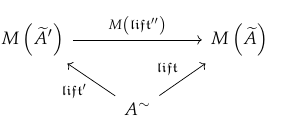
\includegraphics[width=0.5\textwidth]{Covering.png}
	%		\caption{A boat.}
	%		\label{fig:boat1}
\end{figure}
		

			\end{definition}
		where $M\left( \lift''\right)$ is the unique extension of $\lift''$.
If the universal covering exists then  the \alert{fundamental group} of $A$ is given by
\be\label{fund_eqn}
\pi_1\left(A \right) \bydef G\left(\left.\widetilde{A} \right| A\right)
\ee
where $G\left(\left.\widetilde{A} \right| A\right)$ is the covering group (cf. Definition \ref{covering_defn}).

\end{frame}


\section{$C^*$-algebra of compact operators}
\begin{frame}
If $\sH$ is a Hilbert space and $A = \K\left(\sH \right)$ then for any  left ideal $L\subset $ there is a closed $\C$-linear subspace $V_L \subset \K\left(\sH \right)$ such that
\bean
L = \left\{\left.a \in \K\left(\sH \right)\right| a V_L = \{0\}\right\}.
\eean
If $L$ is maximal then $V_L$ is a one dimensional space. Any ultrafilter is principal, generated by maximal ideal. The set of one-dimensional subspaces of $\sH$ is a complex projective space  $\C P\left(\sH \right)$, i.e. there is the natural set theoretic bijective map  $\mathfrak{Gelfand}\left(\K\left(\sH \right) \right)\cong  \C P\left(\sH \right)$. The topology  of $\mathfrak{Gelfand}\left(\K\left(\sH \right)\right) $ contains all sets $\C P\left(\sH \right) \setminus V$ where $V$ is a linear projective  $\C$ subspace of  $\C P\left(\sH \right)$. The identity map yields the  continuous map 
$$
\phi_{\sH} : \C P\left(\sH \right)_{\mathfrak{Hausdorff}}\to \C P\left(\sH \right)_{\mathfrak{Gelfand}}
$$
where $\C P_{\mathfrak{Hausdorff}}\left(\sH \right) $ is the projective  space with   Hausdorff  topology and  $\C P\left(\sH \right)_{\mathfrak{Gelfand}}$ is the same set  with the topology of the Gelfand space.
\end{frame}
\begin{frame}
If $\dim \sH = n < \infty$  then $\C P\left(\sH \right)= \C P^n$ and there is the \alert{Zariski topology} on $ \C P^n$ such that closed subsets are given by polynomial equations. The closed sets of the Gelfand space are given by linear equations, so the Zariski topology is finer then Gelfand one.
There is a composition of continuous maps
$$
\C P^n_{\mathfrak{Hausdorff}}\to \C P^n_{\mathfrak{Zariski}}\to \C P^n_{\mathfrak{Gelfand}}
$$
where the subscript $_{\mathfrak{Zariski}}$ means the Zariski topology. Any open subset of $\C P^n_{\mathfrak{Zariski}}$ and $\C P^n_{\mathfrak{Gelfand}}$ is dense in $\C P^n_{\mathfrak{Zariski}}$ and $\C P^n_{\mathfrak{Gelfand}}$ respectively. If both $\mathscr A'$ and $\mathscr A''$ are locally constant sheaves on $\C P^n_{\mathfrak{Zariski}}$ and $\C P^n_{\mathfrak{Gelfand}}$ then
\bean
p > 0 \quad \Rightarrow\quad  H^p\left( \C P^n_{\mathfrak{Zariski}}, \mathscr A'\right) = H^p\left( \C P^n_{\mathfrak{Gelfand}}, \mathscr A''\right) = \{0\}.
\eean

\end{frame}
\begin{frame}
\begin{theorem}\alert{Ivankov}
If $\C P^n_{\mathfrak{Zariski}}\xrightarrow{f} \C P^n_{\mathfrak{Gelfand}}$  is the natural continuous map then and $\mathscr F$ is a coherent sheaf of modules on $\C P^n_{\mathfrak{Zariski}}$ then for any $p\in \N$ there is the natural  isomorphism
\bean
H^p\left( \C P^n_{\mathfrak{Zariski}}, \mathscr F\right) \cong H^p\left( \C P^n_{\mathfrak{Gelfand}}, f_* \mathscr F\right)
\eean 
where $f_* \mathscr F$ is the direct image of $\mathscr F$.
 \end{theorem}
 \section{Synthetic and analytic projective geometry}
\end{frame}
\begin{frame}
 {\Large  Synthetic and analytic projective geometry}
There is the \alert{synthetic projective geometry} given by the system of axioms. The axioms yield \alert{ projective spaces}, its \alert{points}, \alert{lines}, linear subspaces. 
\begin{definition}
	%Definition. 
	Let $V$ be a vector space of dimension $d \ge 3$ over a division ring
	$F$. We define the rank 2 geometry $\mathbb{P}(V)$ as follows:
	\begin{itemize}
		\item the points of $\mathbb{P}(V)$ are the 1-dimensional subspaces of $V$,
		\item the lines of $\mathbb{P}(V)$ are the 2-dimensional subspaces of $V$,
		\item the incidence of  $\mathbb{P}(V)$ is set-theoretical containment.
	\end{itemize}
\end{definition}
\begin{theorem}
	%2.1.1 Theorem. 
	Let $V$ be a vector space of dimension $d \ge 3$ over a division
	ring $F$. Then $\mathbb{P}(V)$ is a projective space. We call $\mathbb{P}(V)$  the projective space
	coordinatized by $F$,
\end{theorem}
The above theorem states a one-to-one correspondence between \alert{synthetic and analytic projective geometry}.
\end{frame}
  \section{Topological projective geometry}
 \begin{frame}
  {\Large  Topological projective geometry}
  		\begin{definition}\label{top_irreducible_defn}
  	%5.1.1. Definition. 
  	%	Definition. 
  	A nonempty subset $\sY$ of a topological space $\sX$ is \alert{ irreducible} if 
  	it cannot be expressed as the union $\sY = \sY_1 \cup \sY_2$ of two proper subsets, each one of which is closed in $\sY$. The empty set is not considered to be 
  	irreducible. 
  \end{definition}
  \begin{definition}\label{top_dimension_defn}
  	If $\sX$ is a topological space, we define the \alert{ dimension} of $\sX$ (denoted 
  	$\dim \sX$) to be the supremum of all integers $n$ such that there exists a chain 
  	\bean
  	\sZ_0 \subsetneqq	\sZ_1 \subsetneqq...\subsetneqq	\sZ_n 					\eean 
  	of distinct irreducible closed subsets of $\sX$.
  \end{definition} 
Any Gelfand space $\C P^n_{\mathfrak{Gelfand}}$ yields a \alert{topological projective geometry} where points are elements of $\C P^n_{\mathfrak{Gelfand}}$, lines are one-dimensional subspaces of $\C P^n_{\mathfrak{Gelfand}}$, etc.
 \end{frame}
  \begin{frame}
 	
 \begin{definition}
 	Let $\sV, ~\sV'$ be vector spaces over $K, K'$. a map $f: \sV \to \sV'$ is called \alert{ semilinear} if there exists an automorphism $\sigma :K \to K'$ such that
 	\bean
 	f\left(\la x + \mu y \right) = \sigma\left(\la \right) f\left( x\right) + \sigma\left(\mu \right) f\left( y\right) 
 	\eean
 	for all $x, y\in \sV$, $\la, \mu \in K$. If $\sX, \sX'$ are affine spaces over $K, K'$ a map $f: \sX \to \sX'$ is called \alert{ semiaffine} if there exists $a \in \sX$ such that $\overline f: \sX_a \to \sX_{f\left(a \right) }$ is semilinear.
 	
 \end{definition}
 
   \end{frame}
  \begin{frame}
  	 \begin{theorem}
  		Let $\sX$, $\sX'$ be affine spaces of same finite dimension $d \ge 2$. Let $f: \sX \to \sX'$ be a bijection which takes any three collinear points $a, b, c \in \sX'$ into  collinear points $f(a), f(b), f(c)\in \sX'$. Then $f$ is semiaffine
  	\end{theorem}
  \begin{definition}\label{collineatioin_defn}
  	A \alert{ collineation} of $P$ is a bijective map from the point set and line set
  	of $P$ onto themselves that preserves incidence.
  \end{definition}
  \begin{theorem}\label{fund_proj_thm}
 	Let both $\mathbb{P}\left( E\right)$,   $\mathbb{P}\left( E'\right)$ two projective spaces of equal dimension  $\ge 2$ over fields $K$ and $K'$. Let $f: \mathbb{P}\left( E\right)\cong \mathbb{P}\left( E'\right)$ be a set theoretic bijection such that for any three collinear points $a, b, c \in \mathbb{P}\left( E\right)$ the points $f(a), f(b), f(c) \in \mathbb{P}\left( E\right)$ are collinear then there is a semilinear map $f : E \to E'$ with $f = \underline{ \hat f}$
 \end{theorem}
   \end{frame}
   \begin{frame}
		\begin{definition}\label{top_irreducible_defn}
	%5.1.1. Definition. 
	%	Definition. 
	A nonempty subset $\sY$ of a topological space $\sX$ is \alert{ irreducible} if 
	it cannot be expressed as the union $\sY = \sY_1 \cup \sY_2$ of two proper subsets, each one of which is closed in $\sY$. The empty set is not considered to be 
	irreducible. 
\end{definition}
\begin{definition}\label{top_dimension_defn}
	If $\sX$ is a topological space, we define the \alert{ dimension} of $\sX$ (denoted 
	$\dim \sX$) to be the supremum of all integers $n$ such that there exists a chain 
	\bean
	\sZ_0 \subsetneqq	\sZ_1 \subsetneqq...\subsetneqq	\sZ_n 					\eean 
	of distinct irreducible closed subsets of $\sX$.
\end{definition}
\end{frame}
\begin{frame}

\begin{definition}\label{top_codimension_defn}
	If $\sZ$ is an irreducible closed subset of $\sZ$, then the 
	\alert{ codimension} of $\sZ$ in $\sX$, denoted $\codim(\sZ,\sX$) is the supremum of integers $n$.
	such that there exists a chain 
	\bean
	\sZ = \sZ_0 \supsetneqq \sZ_1 \supsetneqq... \supsetneqq \sZ_0 \supsetneqq \sZ_n 
	\eean 
	of distinct closed irreducible subsets of $\sX$, beginning with $\sZ$. If $\sY$ is any 
	closed subset of $\sY$, we define 
	\bean
	\codim(\sY,\sX)\bydef \inf_{\sZ \subset \sY} \codim \sZ.
	\eean
	where the infinum is taken over all closed irreducible subsets of $\sY$. 
\end{definition}
 The dimension of any irreducible  closed subset $\sY\subset  \C P^n_{\mathfrak{Gelfand}}$ equals to the dimension of $\sY$ as a projective subspace of $\C P^n_{\mathfrak{Gelfand}}$. There is the one-to-one correspondence between homeomorphisms of $\C P^n_{\mathfrak{Gelfand}}$ and collineations of $\C P^n$, i.e. the topology of $\C P^n_{\mathfrak{Gelfand}}$ uniquely defines a projective structure of $\C P^n$.
 
   \end{frame}
  \section{Chow ring}
  \begin{frame}
  	Homology of smooth manifolds can be calculated using 
  cycles represented by submanifolds are closed homology classes that can be realized by the image of a smooth, often embedded, manifold within a larger manifold. Algebraic geometry has similar construction, i.e. cycles can be represented by algebraic subvarieties.
  	.
  In algebraic geometry, the \alert{Chow groups} (named after Wei-Liang Chow by Claude Chevalley  of an algebraic variety over any field are algebro-geometric analogs of the homology of a topological space. The elements of the Chow group are formed out of subvarieties (so-called algebraic cycles) in a similar way to how simplicial or cellular homology groups are formed out of subcomplexes. When the variety is smooth, the Chow groups can be interpreted as cohomology groups (compare Poincaré duality) and have a multiplication called the intersection product. The Chow groups carry rich information about an algebraic variety. If we consider a complex variety $\sX\subset \C P^n$ then its  Chow groups are naturally isomorphic to cohomology groups $H^*\left( \sX ; \mathbb{Z}\right)$. 
  \end{frame}
  \begin{frame}
\begin{definition}\label{prime_divisor_dern}
	%	Definition. 
 A \alert{ prime divisor} on $\sX$ is a closed integral subscheme $\sY$ of codimension one. A \alert{ Weil divisor} is an element of the free Abelian group $\mathrm{Div}\sX$ generated by the prime divisors. We write a divisor as $D =\sum_{j=1}^n n_j \sY_j $  where the $\sY_j$ are prime divisors, the $n_j$ are integers, and 
	only finitely many $n_j$ are different from zero. If all the $n_j \ge 0$, we say 
	that $D$ is \alert{ effective}. 
\end{definition}
Algebraic geometry operates with equivalence relation on the group of divisors. Two divisors are 
\alert{linearly equivalent} if they differ by a sum 
\be\label{projective_sum_eqn}
\sum n_\iota \left(\left[\sV_\iota\left(0 \right) \right]- \left[\sV_\iota\left(\infty \right) \right] \right) 
\ee 
with $n_\iota$, integers, $\sV_\iota$ subvarieties of $\sX \times \C P^1$ whose projections to $\C P^1$ are dominant, 
and $\sV_\iota\left(0 \right)$ and $\sV_\iota\left(\infty \right)$ are the scheme-theoretic fibres of $\sV$, over $0$ and $\infty$, regarded 
as subschemes of $\sX \cong \sX\left(0 \right)$  and $\sX \cong \sX\left(\infty \right)$. 
  \end{frame} 
  \begin{frame}
 Let $\sX$ be any variety over field  $k$. A \alert{ cycle of codimension} $r$ on $\sX$ is an element 
 of the free Abelian group generated by the closed irreducible subvarieties of $\sX$ 
 of codimension $r$. So we write a cycle as $\sY = \sum n_j \sY_j$ where the $\sY_j$ are subvarieties, and $n_j \in \mathbb Z$. 
 Let $f: \sX \to \sX'$ be a morphism of varieties, and let $\sY$ be a subvariety of $\sX$. 
 If $\dim f\left(\sY \right) < \dim \sY$, we set $f_*\left( \sY\right)= 0$ . If $\dim f\left(\sY \right) = \dim \sY$, then the 
 function field $K\left(\sY \right)$  is a finite extension field of $K\left(f\left( \sY \right) \right)$, and we set 
 $$
 f\left( \sY\right)\bydef \left[K\left(\sY \right):K\left(f\left( \sY\right)  \right)\right]\cdot \overline{f\left(\sY \right) } 
 $$
 	Extending by linearity defines a homomorphism  $f_*$ of the group of cycles on $\sX$
 to the group of cycles on $\sX'$.	  
 Now we come to the definition of rational equivalence For any subvariety 
 $\sV$ of $\sX$, let $f: \widetilde \sV\to \sV$ be the normalization of $\sV$.\end{frame}
 
 \begin{frame}
  Whenever $D$ and $D'$ are linearly equivalent Weil divisors on V, we say 
 that $f_*D$ and $f_*D'$ are \alert{ rationally equivalent} as cycles on $\sX$. Then we define 
 rational equivalence of cycles on X in general by dividing out by the group 
 generated by all such $f_*D'\sim f_*D'$ for all subvarieties $\sV$, and all linearly 
 equivalent Weil divisors $D, D'$ on $\sV$. In particular, if $\sX$  itself is normal, then 
 rational equivalence for cycles of codimension 1 coincides with linear 
 equivalence of Weil divisors. 
 For each $r$ we let $A^r\left(\sX \right)$  be the group of cycles of codimension $r$ on $\sX$ 
 modulo rational equivalence. We denote by $A\left(\sX\right)= \bigoplus_{r= 0}^n A^r\left( \sX\right)$  the graded group  where $n = \dim \sX$. Note that $A^0\left( \sX\right)= \mathbb Z$ , and that $A^r\left(\sX \right)= 0$  for $r > \dim \sX$.
  \end{frame}
  \begin{frame}
  An intersection theory on an explained in \cite{hartshorne:ag} class of varieties $\mathfrak{B}$ consists of giving a 
  pairing $A^r\left(\sX \right)\times A^s\left(\sX \right)\to A^{r + s}\left(\sX \right)$  for each $r,s$, and for each $\sX \in \mathfrak{B}$, satisfying 
  the axioms listed below. If $\sY \in A^r\left(\sX \right)$ and $\sZ \in A^s\left(\sX \right)$ we denote the intersection cycle class by $\sY.\sZ$. 
  Before stating the axioms, for any morphism  $f : \sX \to \sX'$ of varieties in $\mathfrak{B}$ 
  we assume that $\sX \times \sX'$ is also in $\mathfrak{B}$, and we define a homomorphism 
  $f^*: \left(\sX' \right) \to \left(\sX \right)$ as follows. For a subvariety $\sY'\subset \sY$ we define 
  \bean
  f^*\left(\sY' \right)\bydef p_{1*} \left( \Ga_f. p^{-1}_2\left( \sY'\right) \right) 
  \eean
  where $p_1$ and $p_2$ are the projections of $\sX \times \sX'$ to $\sX$ and $\sX'$, and $\Ga_f$ is the 
  graph of $f$, considered as a cycle on $\sX \times \sX'$. 
  This data is now subject to the following requirements. 
\end{frame}

  \begin{enumerate}
  	\item[A1.] The intersection pairing makes $A\left( \sX\right)$  into a commutative associative 
  	graded ring with identity, for every $\sX \in \mathfrak{B}$. It is called the \alert{ Chow ring} of $\sX$. 
  	\item[A2.] For any morphism $f : \sX \to \sX '$ of varieties in $\mathfrak{B} ~,~ f^*: A(\sX')\to A(\sX)$ is a
  	ring homomorphism. If $f : \sX' \to \sX''$ is another morphism, then $g^* \circ f^* = \left(g \circ f \right)^*$. 
  	\item[A3.] For any proper morphism $f : \sX \to \sX '$ of varieties in $\mathfrak{B}$, $f : \sX \to \sX '$ is a homomorphism of graded groups (which shifts degrees). If 
  	$g : \sX' \to \sX ''$ is another morphism, then  $g_* \circ f_* = \left(g \circ f \right)_*$. 
  	\item[A4.] \alert{ Projection formula}. If $f : \sX \to \sX '$ is a proper morphism, if $x \in  A\left( \sX\right)$  
  	and $y \in  A\left( \sX'\right)$, then 
  	\bean
  	f_*\left(x. f^*y \right) = f_*\left( x\right).y
  	\eean 
  	\item[A5.] \alert{ Reduction to the diagonal}. If $\sY$ and $\sZ$ are cycles on $\sX$, and if $\Dl \sX \to \sX \times \sX$ is the diagonal morphism, then 
  	$$
  	\sY.\sZ = \Dl^*\left(\sY \times \sZ \right)/ 
  	$$
  	\item[A6.] \alert{ Local nature}. If $\sY$ and $\sZ$ are subvarieties of $\sX$ which \alert{ intersect properly} 
  	(meaning that every irreducible component of $\sY \cap \sZ$ has codimension equal 
  	to $\codim \sY + \codim \sZ$), then we can write
  	\bean
  	\sY.\sZ = \sum i\left( \sY, \sZ; \mathcal W_\iota \right) \mathcal W_\iota
  	\eean  
  	where the sum runs over the irreducible components $\mathcal W_\iota$ of $\sY$ and $\sZ$, and where 
  	the integer $i\left( \sY, \sZ; \mathcal W_\iota \right)$ depends only on a neighborhood of the generic point 
  	of $\mathcal W_\iota$ on $\sX$. We call $i\left( \sY, \sZ; \mathcal W_\iota \right)$ the \alert{ local intersection multiplicity} of $\sY$ and $\sZ$
  	along $\mathcal W_\iota$. 
  	\item[A7.] \alert{ Normalization}. If $\sY$ is a subvariety of $\sY$, and $\sZ$ is an effective Cartier 
  	divisor meeting $\sY$ properly, then $\sY.\sZ$ is just the cycle associated to the Cartier 
  	divisor $\sY \cap \sZ$ on $\sY$, which is defined by restricting the local equation of 
  	$\sZ$ to $\sY$ (This implies in particular that transversal intersections of non singular subvarieties have multiplicity 1.) 
  	
  \end{enumerate}
  
  \begin{frame}
  
  \begin{theorem}
  	%Theorem 1.1. 
  %	Let $\mathfrak{B}$ be the class of nonsingular quasi-projective varieties over 
  	a fixed algebraically closed field $k$. Then there is a unique intersection 
  	theory for cycles modulo rational equivalence on the varieties $\sX \in \mathfrak{B}$ which 
  	satisfies the axioms A1-A7 above. 
  \end{theorem}
  \end{frame}
  
  
   \section{Chow ring  of $\C P^n_{\mathfrak{Gelfand}}$}
   
   \begin{frame}
   	Here we use the notation \eqref{projecive_not_eqn}. If we consider $\C P^n_{\mathfrak{Gelfand}}$ with $n \ge 2$ as pure topological space and define \alert{ lines} as irreducible closed subsets (cf. Definition \ref{top_irreducible_defn}) having dimension 1 (cf. Definition \ref{top_dimension_defn}) then from the Theorem \ref{fund_proj_thm} one can prove that $\C P^n_{\mathfrak{Gelfand}}$ has natural structure od the complex projective space in the sense of the analytical geometry. Roughly speaking the topology of $\C P^n_{\mathfrak{Gelfand}}$ naturally defines the analytical geometry and vice versa. The geometry is such that the theorems of Desargues and Pappus hold (cf. \cite{projective_geometry} for details). Moreover from the described in \cite{projective_geometry} results it follows that  any  irreducible closed subsets (cf. Definition \ref{top_irreducible_defn}) having dimension $d$ correspond to the linear inclusion $\C P^d\hookto \C P^n$. Here we construct an analog of the well known in the algebraic geometry  intersection theory (cf. Appendix \ref{intersec_sec}). Similarly to the Definition \ref{prime_divisor_dern} we define a \textit{prime divisor}  as an irreducible closed subset  of $\C P^n_{\mathfrak{Gelfand}}$ (cf. Definition \ref{top_irreducible_defn}) having codimension 1 (cf. Definition \ref{top_codimension_defn}). One can define the group Abelian group $\mathrm{Div}~\C P^n$ which is an analog of $\mathrm{Div}~\sX$ and any divisor correspond to a injective linear map $\C P^{n - 1} \hookto \C P^n$.
   \end{frame}
   \begin{frame}
   There is the natural correspondence between the  set of continuous maps  $\C P^n_{\mathfrak{Gelfand}}\to \C P^1_{\mathfrak{Gelfand}}\cong \C P^n_{\mathfrak{Zariski}}$ and the set of linear in sense of analytical geometry  maps $\C P^n\to \C P^1$. Similarly to the Appendix \ref{principal_div_empt} for any linear map $f: \C P^n\to \C P^1$ one can define an analog of the \alert{ principal divisor} (cf. Definition \ref{principal_div_defn}) given by 
   	$$
   	f\left( 0\right) - f\left(\infty \right). 
   	$$
   \end{frame}
   \begin{frame}
   There is a notion of \alert{ linearly equivalent} divisors (cf. Definition \ref{linearly_div_defn}). For any two different linear maps $\phi' :\C P^{n - 1} \hookto \C P^n$ and $\phi'': \C P^{n - 1} \hookto \C P^n$ there is a linear map $f: \C P^n\to \C P^1$ such that 
   \bean
   f\left(0 \right) = \phi'\left(\C P^{n - 1} \right),\\ 
   f\left(\infty \right) = \phi''\left(\C P^{n - 1} \right),
   \eean 
   i.e. any prime divisors are linearly equivalent so one has 
  \bean
   \mathrm {Cl}~\C P^n_{\mathfrak{Gelfand}}\cong \Z\left[\C P^{n-1}\right]
  \eean
   where $\left[\C P^{n-1}\right]\in \mathrm {Cl}~\C P^n_{\mathfrak{Gelfand}}$ is an analog an element of divisor class group (cf. Definition \ref{linearly_div_defn}) and $\left[\C P^{n-1}\right]$ is the  represented by $\C P^{n-1}\subset \C P^n_{\mathfrak{Gelfand}}$ class. Similarly to the Appendix \ref{ag_cycles_empt} one can define \alert{ cycle of codimension} $r$ on $\sX$ is an element 
   of the free Abelian group generated by the closed irreducible subspaces  of $\C P^n_{\mathfrak{Gelfand}}$ of codimension $r$. If both $\sY', \sY'' \subset \C P^n_{\mathfrak{Gelfand}}$ are two    closed irreducible subspaces  of $\C P^n_{\mathfrak{Gelfand}}$ of codimension $r$ such that the intersection $\sY' \cap \sY''$ has codimension $2r$ then there are:
\end{frame}
\begin{frame}
\begin{enumerate}
	\item [(a)] the natural closed irreducible subspace $\sZ \subset \C P^n_{\mathfrak{Gelfand}}$ of codimension  $r - 1$ with $\sY' \cup \sY''\subset \sX$,
	\item [(b)] a continuous with respect to Gelfand topology  map $f: \sZ \to \C P^1$ with
	\be\label{lc_eq_eqn}
	\sY' = f^{-1}\left(0 \right),
	\sY'' = f^{-1}\left(\infty \right)
	\ee 
\end{enumerate}
i.e. cycles are \alert{ rationally equivalent}. So similarly to thr Appendix  \ref{linearly_div_defn} there are the group $A^r\left(\C P^n_{\mathfrak{Gelfand}} \right)$ of rationally equivalent  classes of $r$-cycles. From \eqref{lc_eq_eqn} it follows that the cycled $\sX'$ and $\sX'$ are rationally equivalent, i.e.
\be\label{ar_c_eqn}
\left[\sX'\right]= \left[\sX''\right]\in A^r\left(\C P^n_{\mathfrak{Gelfand}} \right).
\ee
Using the equation \eqref{ar_c_eqn} one can deduce that for any $r = 0,..., n$ there is the natural isomorphism
\be
A^r\left(\C P^n_{\mathfrak{Gelfand}} \right) = \Z \left[\C P^{n-r}\right]
\ee
where  $\left[\C P^{n-r}\right]$ is represented by a cycle $\C P^{n-r} \subset \C P^n_{\mathfrak{Gelfand}}$.
\end{frame}
\section{The ring structure}
\begin{frame}
Any $m$-dimensional irreducible subspace  of $\C P^n_{\mathfrak{Gelfand}}$ can be represented by an element of the set
$$
L^m_n \bydef \left\{\left.\psi \in \Hom_\C\left(\C^{m + 1}, \C^{n+1}  \right) \right| \rank \psi = m + 1 \right\}\subset \Hom_\C\left(\C^{m + 1}, \C^{n+1}  \right).
$$
where $\Hom_\C\left(\C^{m + 1}, \C^{n+1}  \right)$ is the  $\C$-linear space of  $\C$-linear homomorphisms. There is the \alert{ Gelfand  topology} on $\Hom_\C\left(\C^{m + 1}, \C^{n+1}  \right)$ which is the minimal among the topologies such that any $\C$-linear subspace of $\Hom_\C\left(\C^{m + 1}, \C^{n+1}  \right)$ is closed. This topology yields the natural (Gelfand) topology on both $L^m_n$ and the set $C^m_n$ of $m$-dimensional irreducible subspace  of $\C P^n_{\mathfrak{Gelfand}}$ (cf. Definitions \ref{top_final_defn} and \ref{top_init_defn}). If $\sY' \in C^{m'}_n$ then there is an open dense subset $\sU^{m''}_n \subset C^{m''}_m$ such that
\be\label{gen_pos_eqn}
\forall \sY'' \in \sU^{m''}_n \quad \sY' \cap \sY'' \cong \C P^{n - m' - m''}
\ee
\end{frame}
\begin{frame}
We say that the hypothesis \eqref{gen_pos_eqn} is the \textit{general position} (cf. Remark \ref{gen_pos_eqn}). Similarly to the Appendix \ref{ag_cycles_empt} we define the ring structure on $\C P^n_{\mathfrak{Gelfand}}$ such that
\be
\left[\C P^{n-m'}\right]\cdot \left[\C P^{n-m''}\right]= \left[\C P^{n-m'-m''}\right]
\ee
From out construction one has the natural isomorphism
$$
A\left( \C P^n_{\mathfrak{Gelfand}}\right) \cong \Z\left[\left[\C P^1\right]\right] /\left( \left[\C P^{n-1}\right] \right)^{n+1}
$$
There is the following mapping between Zariski and Gelfand topology.
\end{frame}
\section{Cobordism interpretation}
\begin{frame}
\begin{definition}\label{cobordism_category_defn}
	A \textit{cobordism category} $\left(\mathscr C, \partial, j\right)$ is a triple in which
	\begin{enumerate}
		\item [(a)] $\mathscr C$ is a category having finite sums and an initial object;
		\item[(b)] $\partial:  \mathscr C \to \mathscr C$ is an additive  functor such that for each object $X$ of $\mathscr C$, $~\partial \partial \left( X\right)$ is the initial object;
		\item[(c)] $j :\partial \to \Id_{\mathscr C}$ is a natural transformation of additive from $\partial$ to the identity functor $\Id_{\mathscr C}$; and 
		\item[(d)] There is a small category $\Id_{\mathscr C_0}$ or $\Id_{\mathscr C}$ such that each object of $\mathscr C$ is isomorphic  to an object of $\mathscr C_0$.
	\end{enumerate} 
\end{definition}
\end{frame}
\begin{frame}
There is an interpretation of the Chow ring it terms of the cobordism category (cf. Definition \ref{cobordism_category_defn}).
Let $n \in \N$, and let $\mathscr{L}\left(n \right) $ be a category such that
\begin{itemize}
	\item any  $\mathscr{L}\left(n \right)$-object is a pair $\left(\sX, f \right)$ where $\sX \subset \C P^n_{\mathfrak{Gelfand}}$ is an irreducible closed subset and $f: \sX \to \C P^1_{\mathfrak{Gelfand}}\cong \C P^1_{\mathfrak{Zariski}}$ is a continuous map with $0 \in f\left( \sX\right)$. 
		\begin{figure}
		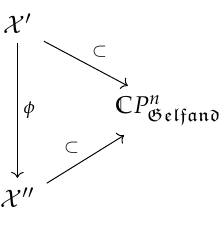
\includegraphics[width=0.4\linewidth]{cobord.png}
		%		\caption{A boat.}
		%		\label{fig:boat1}
	\end{figure}
	
	\item an arrow from $\left(\sX', f' \right)$ to $\left(\sX'', f'' \right)$ is an injective  continuous  map $\phi: \sX' \hookto \sX''$ satisfying to the following conditions:
\end{itemize}
\end{frame}
\begin{frame}
Let $\mathscr{C}\left(n \right)$ be a category (cf. Definition \ref{category_defn}) such that
be a category such that
\begin{itemize}
	\item any object of $\mathscr{C}\left(n \right)$ is a $\Z$-linear combination of $\mathscr{L}\left(n \right)$ objects,
	\item if $f_1, ..., f_{m'}, g_1, ..., g_{m''}$ are $\mathscr{L}\left(n \right)$-objects then there is the unique  $\mathscr{C}\left(n \right)$-arrow from $\sum_{j = 1}^{m'}c_j f_j$ to $\sum_{\iota = 1}^{m''}d_\iota g_\iota$ with integer $c_\iota, ~d_\iota$ if and only if for any $\iota' \in 1,..., m'$ there is  $\iota'' \in 1,..., m''$ and $\mathscr{L}\left(n \right)$-arrow $f_{\iota'}\xrightarrow{\phi} g_{\iota''}$.
\end{itemize}
So the set of $\mathscr{C}\left(n \right)$ objects is the Grothendieck group of the category $\mathscr{L}\left(n \right)$.
We suppose that there is the natural two=point subset $\left\{0, \infty\right\}\subset \C P^1$. For any $\mathscr{L}\left(n \right)$-object $\left(\sX, f \right)$ we define two objects $\left(\sX_0\bydef f^{-1}\left(0 \right) , f_0 \right)$  and $\left(\sX_1\bydef f^{-1}\left(\infty \right) , f_1 \right)$ where $f_0\left(\sX_0 \right) = f_1\left(\sX_1 \right)= {0} \in \C P^1_{\mathfrak{Gelfand}}$. If $\sX_1 = \emptyset$ then we set $f_1\left(\sX_1 \right)= \emptyset$.
If $1_\Z \cdot \left(\sX, f \right)$ is $\mathscr{C}\left(n \right)$-object then we define
\be\label{co_d_eqn}
\partial \left( 1_\Z \cdot \left(\sX, f \right)\right)  \bydef \begin{cases}
	1_\Z \cdot \left(\sX_0, f_0 \right) - 1_\Z \cdot \left(\sX_1, f_1 \right) & \infty \in f\left(\sX \right) \\
	0_{\mathscr{C}\left(n \right)} &  \infty \notin f\left(\sX \right)
\end{cases}
\ee 
The $\Z$-linearity yields the unique additive  functor $\mathscr{C}\left(n \right)\xrightarrow{\partial} \mathscr{C}\left(n \right)$.
\end{frame}
\begin{frame}
\begin{lemma}
	Under the above hypothesis  $\mathscr{C}\left(n \right)$ is the cobordism category.
\end{lemma}

\begin {table}[H]
\caption {Mapping between Zariski and Gelfand topology } \label{main_mapping_table} 
	\begin{tabular}{|c|c|c|}
		\hline
		&	 Gelfand topology &  Zariski topology\\
		\hline
		& & 	\\
		The space & $\C P^n_{\mathfrak{Gelfand}}$ &  $\C P^n_{\mathfrak{Zariski}}$ \\
		&&	\\
		Cycles 	&	Linear subspace  & Algebraic subvariety \\
		& $\C P^m \subset \C P^n$ & $\sX \subset \C P^n$	\\
		& &\\
		Equivalence  & Cobordism & Rational equivalence\\
	relation	&& \\
	&& \\
		Chow ring	& $\Z\left[\left[\C P^{n-1}\right]\right] /\left( \left[\C P^1\right] \right)^{n+1}$	& $\Z\left[\left[\C P^1\right]\right] /\left( \left[\C P^{n-1}\right] \right)^{n+1}$\\
		&& \\
		\hline
	\end{tabular}
\end {table}
\end{frame}


\section{Hausdorff blowing-up}
\begin{frame}
	\begin{definition}\label{blowing_defn}
	If $A$ is a $C^*$-algebra then any good $*$-homomorphism  $\mathfrak {Blowing}_{\sX-A }:C_0\left( \sX\right) \hookto M\left(A \right)$  (or equivalently $C_0\left( \sX\right) \subset M\left(A \right)$ ) is \alert{Hausdorff blowing-up}.
\end{definition}
	\begin{rem}
The "blowing-up" word is inspired by following reasons:
\begin{itemize}
	\item Sometimes there is  the natural partially defined  surjective  map from  Hausdorff blowing-up to the spectrum.
	\item  In the algebraic geometry   "blowing-up" means  excluding of singular points.
\end{itemize}
\end{rem}
\end{frame}
\section{Universal blowing-up}
\begin{frame}
	If $A$ is a $C^*$-algebra and  $C_0\left( \sX\right) \to M\left(A \right)$ is Hausdorff blowing-up then the action $C_b\left(
\sX \right) \times C_c\left(\sX \right)\to  C_c\left(\sX \right)$ yields  the action $C_b\left(
\sX \right) \times\left(  C_c\left(\sX \right) A\right) \to  C_c\left(\sX \right)A$. Since $  C_c\left(\sX \right)A$ is dense in $A$ one the action $C_b\left(
\sX \right) \times\left(  C_c\left(\sX \right) A\right) \to  C_c\left(\sX \right)A$ can be naturally extended up to the action $C_b\left(
\sX \right) \times A \to  A$. Similarly one has the natural right action $A \times C_b\left(
\sX \right) \to  A$. One can prove that both these actions yield an inclusion
\be\label{blowing_b_eqn} 
C_b\left(\sX \right)\to M\left(A \right).  
\ee
\end{frame}
\begin{frame}
\begin{definition}\label{hausdorff_defn}
	Let $\sX$ be a topological space. The $\sX$-\alert{ Hausdorff category}  $\mathfrak{Hausdorff}\left( \sX\right)$ is such that 
	
	\begin{itemize}
		\item objects of $\mathfrak{Hausdorff}\left( \sX\right)$ are continuous surjective maps $\sX \onto \sY$ onto Hausdorff locally compact  space $\sY$, 
		\item a morphism form $\sX \onto \sY'$ to $\sX \onto \sY''$ is a continuous surjective map  $\sY' \onto \sY''$ such that the diagram 
			\begin{figure}
		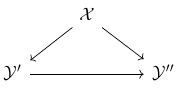
\includegraphics[width=0.4\linewidth]{hauscat.png}
		%		\caption{A boat.}
		%		\label{fig:boat1}
	\end{figure}
		
		is commutative.
	\end{itemize}
	
\end{definition}
\begin{lemma}
	For any topological space $\sX$ there is the initial object  of the  $\sX$-{Hausdorff category}.
\end{lemma}

\end{frame}
\begin{frame}
	\begin{proof}
		Let $A$ be a commutative $C^*$-algebra of all bonded continuous maps from $\sX$ to $\C$ and let $\sY'$ be the spectrum of $A$ (cf. Definition \ref{spectrum_prime_primtive_defn}).  Any $x \in \sX$ yields the maximal ideal 
		$$
		I_x \bydef \left\{ f \in A | f\left( x\right) = 0\right\}
		$$
		The ideal $I_x$ yield a point $y \in \sY'$. So there is the natural  map $\phi' :\sX \to \sY'$. If $\sY \bydef \phi'\left( \sX\right)$ then $\phi'$ yields  the surjective map  $\phi :\sX \onto \sY$. One can prove that the map is continuous. It turns out that the spaces $\sY'$ and $\sY$ are locally compact  and Hausdorff.  If there is and an object $\sX \onto \sY''$ with nonidentical morphism $\phi'' : \sY''\onto \sY$ then there are $y_1, y_2 \in \sY''$ with $y_1 \neq y_2$ and $\phi''\left( y_1\right) = \phi''\left( y_2\right)$. There is $f \in C_0\left( \sY''\right)$ such that $f\left( y_1\right)  \neq f\left( y_2\right)$. Clearly $f \in A$ but $f \notin C_0\left(
		\sY \right)$ i.e. $C_0\left(\sY \right)  \subsetneqq A$. It is a contradiction which proves that the existence jf $\sY''$ is impossible.  
			\end{proof}
\end{frame}
\begin{frame}
	\begin{definition}\label{blowing_uni_h_defn}
	The initial object of the category $\sX$-{Hausdorff category} is the	$\sX$ - \alert{universal Hausdorff quotient space}.
\end{definition}	

\begin{lemma}\label{final_blowing_lem}
	Let $A$ be a $C^*$-algebra. If  a category $\mathfrak{Blowing}\left(A\right)$  such that 
	\begin{enumerate}
		\item[(a)] any object of $\mathfrak{Blowing}\left(A\right)$ is Hausdorff blowing-up, 
		\item[(b)] a morphism from $C_0\left( \sX'\right) \hookto M\left(A \right)$ to $C_0\left( \sX''\right) \hookto M\left(A \right)$ is an injective *-homomorphism $C_b\left( \sX'\right) \hookto C_b\left( \sX''\right)$ such that the diagram 
		such that the diagram 			\begin{figure}
			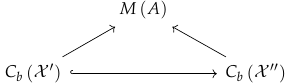
\includegraphics[width=0.6\linewidth]{unibl.png}
			%		\caption{A boat.}
			%		\label{fig:boat1}
		\end{figure}
		
		is commutative.
	\end{enumerate}
	then there is the final object $\mathfrak{Blowing}\left(A\right)$.
	\end{lemma}
	
\end{frame}
\begin{frame}
\begin{proof}
	If $\sY$ is the $\mathfrak{Gelfand}\left( A\right)
	$ {universal Hausdorff quotient space} and $C_0\left( \sX'\right) \to M\left(\sX  \right)$ is Hausdorff blowing-up, then   there are:
	\begin{itemize}
		\item the natural surjective continuous map $\sY \to \sX$,
		\item The natural  inclusion $C_0\left(\sX \right)\subset C_b\left(\sY \right)$. 
	\end{itemize}
	If $\left\{C_0\left(\sX_\la \right) \right\}_{\la \in \La}$  is family of all Blowing-ups then the $C^*$-norm completion of the included into  $C_b\left(\sY \right)$ union $\bigcup_{\la\in \La} C_0\left(\sX_\la \right)$ is a commutative $C^*$-algebra $C_0\left( \sX\right)$. One can proof that the natural inclusion  $C_0\left(\sX \right) \subset M\left( A\right)$ is the final object of the category  $\mathfrak{Blowing}\left(A\right)$.
\end{proof}
\begin{definition}\label{blowing_universal_defn}
	The final object of the category $\mathfrak{Blowing}\left(A\right)$  of this category $C_0\left( \sX\right) \hookto M\left(A \right)$ is  \alert{universal Hausdorff blowing-up of} $A$.
\end{definition}	
\end{frame}
\begin{frame}
\begin{definition}\label{blowing_ideals_au_ua_defn}
	Let  $ C_0\left( \sY\right)\subset  M\left( A\right) $ be  Hausdorff blowing-up of $A$ (cf. Definition \ref{blowing_defn}), and let $\sU \subset \sY$ be an open subset. Both   left and right  closed ideals $A_\sU$  and $_\sU A$ of $A$ generated by sets 	$AC_0\left( \sU\right)$ and $C_0\left( \sU\right)A$ are the \alert{left} $\sU$-\alert{ideal} and the \alert{right} $\sU$-\alert{ideal} respectively. A hereditary $C^*$-subalgebra of $A$
	\be\label{blowing_hereditary_u_eqn} 
	\begin{split}
		_\sU A_\sU \bydef	~	_\sU A\cap  A_\sU = A^*	_\sU \cap  A_\sU\\ %(\text{cf. Definition \ref{hered_defn} and the Lemma \ref{hered_bab_lem}}).
	\end{split}
	\ee	
	is the $ \sU$-\alert{subalgebra}.
	
\end{definition}
	\begin{definition}\label{blowing_support_defn}
	If $C_0\left( \sY\right) \subset M\left(A \right)$ is    {Hausdorff blowing-up} of $A$,  $a \in A$ and
	$
	\sU_a \bydef\bigcap 
	\left\{\left.{\sU} \subset \sX\right| a\in~_\sU A_{\sU} \right\}
	$
	then the  closure $\sV_a$  of $\sU_a$ is said to be the \alert{support} of $a$. We write $\supp~ a \bydef \sV_a$.
\end{definition}
\end{frame}
\begin{frame}
	\begin{lemma}\label{blowing_pedersen_compact_lem}
	If  $C_0\left( \sY\right)\hookto M\left( A\right)$ is Hausdorff blowing-up and $a\in A$ belongs to the Pedersen's ideal $K\left(A \right)$  then the support of $a$  is compact.
\end{lemma}
	From the above Lemma it follows that the injective homomorphism $\varphi_\sY : C_0\left(\sX \right) \hookto M\left(A \right)$ is good. So there is the natural surjective continuous map
\bean
\phi_A : \mathfrak{Gelfand}\left(A \right) \to \sY.
\eean
\end{frame}


\section{Continuous trace $C^*$-algebras}
\begin{frame}
\begin{definition}\label{abelian_element_defn}
	A positive element in $C^*$ - algebra $A$ is \alert{ Abelian} if subalgebra $xAx \subset A$ is commutative.
\end{definition}
\begin{definition}\label{continuous_trace_c_alt_defn}
	%Definition 5.13. 
	A \alert{continuous-trace} $C^*$-\alert{algebra} is a $C^*$-algebra $A$ with Hausdorff
	spectrum $\sX$ such that, for each $x_0\in\sX$ there are a neighbourhood $\sU$ of $x_0$ and $a\in A$ such that $\rep_{ x}\left( a\right) $ is a rank-one projection for all $x \in \sU$.
	\end{definition}
	\begin{empt}
If $A$ is a continuous-trace $C^*$-algebra then from Dauns-Hofmann theorem it follows that one has Hausdorff blowing-up
\bean
C_0\left( \sX\right)\hookto M\left( A\right)
\eean 
where $\sX$ is the spectrum of $A$.
	\end{empt}
	\end{frame}
	\begin{frame}

		Let   $A$  be a {continuous-trace} $C^*$-{algebra} with the spectrum $\sX$, and let
\bean
\mathfrak{Comm}\left( A\right)  \text{ is a set of all commutative } C^*\text{-subalgebras of } A.
\eean
Then there is a presheaf  $\mathscr P_{\sX\text{-}A}$  of sets such that for any open $\sU \subset \sX$  one has
\bean
\begin{split}
	\mathscr P_{\sX\text{-}A}\left(\sU \right)\bydef \left\{ C \in	\mathfrak{Comm}\left( A\right) \left|~ C \subset ~_\sU A_\sU \right. \right\};\\
	\rho_{\sU\sV} : \mathscr P_{\sX\text{-}A}\left(\sU \right)\to \mathscr P_{\sX\text{-}A}\left(\sV \right),\\
	C \mapsto C \cap ~_\sV A _\sV.
\end{split}
\eean
and let $\mathrm{Sp\acute{e}}\left(\mathscr P_{\sX\text{-}A} \right)$ be the \'espace etal\'e of the presheaf $\mathrm{Sp\acute{e}}\left(\mathscr P_{\sX\text{-}A} \right)$  with the natural local homeomorphism $p_{\mathrm{Sp\acute{e}}\left(\mathscr P_{\sX\text{-}A} \right)} : \mathrm{Sp\acute{e}}\left(\mathscr P_{\sX\text{-}A} \right) \onto \sX$.
	\end{frame}
	\begin{frame}
		\begin{theorem}\label{ctr_gelfand_thm}
			If $A$ is a {continuous-trace} $C^*$-{algebra}  with the spectrum $\sX$ then there is the natural bijective set theoretic map $\phi_{\mathscr P}:\mathfrak{Gelfand}\left( A\right) \cong \mathrm{Sp\acute{e}}\left(\mathscr P_{\sX\text{-}A} \right)$  with the following commutative diagram
			\begin{figure}
	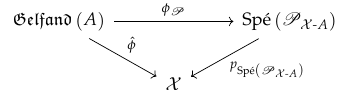
\includegraphics[width=0.6\linewidth]{ctretale.png}
	%		\caption{A boat.}
	%		\label{fig:boat1}
\end{figure}
			where $\hat \phi$ is a specialization of the continuous map from the Gelfand space to the spectrum.
		\end{theorem}	
	\end{frame}
	\begin{frame}
\begin{definition}\label{bicommutant_defn}
	Let $A$ be a $C^*$-algebra. If $\xi \in \mathfrak{Gelfand}\left(A \right)$ and the set
	\bean
	\xi'' \bydef \left\{\left. a \in \rep_{\hat \phi\left( \xi\right) }\left(A \right)\right| \forall L \in \xi \quad  a^* \rep_{\hat \phi\left( \xi\right) }\left(L \right) = \{0\}
	\right\}\subset \rep_{\hat \phi\left( \xi\right) }\left(A \right)
	\eean
	is a proper left ideal of $\rep_{\hat \phi\left( \xi\right) }\left(A \right)$ then $\xi''$ is the \alert{bicommutant} of $\xi$. If for any $\xi \in \mathfrak{Gelfand}\left(A \right)$ the bicommutant exists then there is 
	is the natural surjective  map 
	\bean
	\mathfrak{Gelfand} \left(A \right) \xrightarrow{\phi''}  \mathfrak{Gelfand} \left(A \right)''
	\eean
	where $\mathfrak{Gelfand} \left(A \right)''$ is the set of all bicommutants. We consider the final with respect to the map $\phi''$   topology on $\mathfrak{Gelfand} \left(A \right)''$ and say that the space $\mathfrak{Gelfand} \left(A \right)''$ is the \alert{bicommutant} of $\mathfrak{Gelfand} \left(A \right)$.
	\end{definition}	
\end{frame}
\begin{frame}
	\begin{prop}\alert{Dixmier–Douady}
		%Proposition 5.59. 
		%Theorem 9.9 
		Any stable separable algebra $A$ of continuous
		trace over a second-countable locally compact Hausdorff space $\sX$ is isomorphic to
		$\Ga_0\left( \sX, \A\right)$ , the sections vanishing at infinity of a locally trivial bundle of algebras
		over $\sX$, with fibres $\K$ and structure group $\Aut(\K) = PU = U/\T$. Classes of
		such bundles are in natural bijection with the \v{C}ech cohomology group $\check{H}^3\left(\sX, \Z \right)$.
		The 3-cohomology class $\dl\left( A\right)$  attached to (the stabilization of) a continuous-trace
		algebra A is called its Dixmier–Douady class.
	\end{prop}
	\begin{theorem}\alert{Ivankov}
	Suppose that $A$ is the given by the above proposition   locally trivial   fibre bundle $\F$ with fibre $\K = \K\left(\sH \right)$. There is a subbundle $\E \subset \F$ such that fibers of $\E$ are  rank-one positive operators. It gives a locally trivial bundle $\C P\left(\E \right)\xrightarrow{\phi_\E} \sX$ such that any fibre of $\phi_\E$ is a complex projective space $\C P\left(\sH \right)$. Then there is  the natural set theoretic bijective map
\bean
\phi_C: \C P\left(\E \right)\cong  \mathfrak{Gelfand}\left(A \right)''.
\eean
\end{theorem}	
\end{frame}
\begin{frame}
Under the hypothesis of the above theorem is the natural bijective continuous map 
\bean\label{ctr_bundle_eqn}
\C P\left(\E \right)_{\mathfrak{Hausdorff}}\xrightarrow{\phi_{\C P\left( \E\right) }} \C P\left(\E \right)_{\mathfrak{Gelfand}}
\eean
where $\C P\left(\E \right)_{\mathfrak{Hausdorff}}$ is the set $\C P\left(\E \right)$ having well known Hausdorff topology, and $\C P\left(\E \right)_{\mathfrak{Gelfand}}$ has a topology induced by the natural set theoretic bijective map
$
\phi_C: \C P\left(\E \right)\cong  \mathfrak{Gelfand}\left(A \right)''.
$  The topological invariants of $\C P\left(\E \right)_{\mathfrak{Hausdorff}}$ are well known. The invariants of $\C P\left(\E \right)_{\mathfrak{Gelfand}}$ should be developed. Theory of motives is a good prototype for the theory of invariants of  $\C P\left(\E \right)_{\mathfrak{Gelfand}}$.
\end{frame}
	\section{Classical and quantum projective modules}
	\begin{frame}
\begin{definition}\label{projection_equivalences_defn}
	%Definition 5.2.1. 
	Projections $p$ and $q$ in a $C^*$-algebra $A$ are said to be 
	\begin{itemize}
		\item\alert{ equivalent}, denoted $p\sim q$, when $p = v^*v$ and $q = vv^*$,  $v\in A$ being 
		a partial isometry; 
		\item\alert{ unitarily equivalent}, denoted $p\sim_uq$, when $p = u^*qu$, $u \in A^+$l 
		being unitary; 
		\item\alert{ homotopic}, denoted $p \sim_h q$, when $p$ and $q$ are connected by a norm 
		continuous path of projections in $A$. 
	\end{itemize}
	
\end{definition}
\begin{definition}\label{projection_equivalence_defn}
	%Definition 6.1.1. 
	Call projections $p, q \in \mathbb{M}_\infty\left(A \right)$ \alert{ equivalent}, denoted $p\sim q$, when there is a $v \in \mathbb{M}_\infty\left(A \right)$ such that $p = v^*v$ and $q = vv^*$ 
	The equivalence classes are denoted $[\cdot]$ and the set of all these is 
	\be
	V\left(A \right) \bydef \left\{[p]\left| p = p^* = p^2\in \mathbb{M}_\infty\left(A \right)\right.\right\}
	\ee
	
	\alert{ Addition} in $V\left( A\right)$ is defined by 
	\bean
	[p] + [q] = \left[p' \oplus q'\right]
	\eean
	if $p' \sim p$, $q' \sim  q$, $p'\perp q'$. 
\end{definition}
	\end{frame}
\begin{frame}
If $A$ is a $C^*$-algebra and  $C_0\left( \sX\right)\subset M\left(A\otimes \K \right)$ is universal Hausdorff blowing-up  then there is a  homomorphism 	$\mathfrak{Blowing}^+_{\sX-A\otimes \K }:C\left( \sX^+\right) \hookto M\left(A\otimes \K \right)$ and there is a diagram

	\begin{figure}
	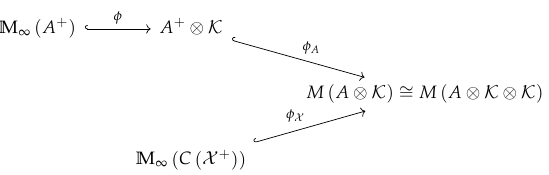
\includegraphics[width=0.9\linewidth]{pmodules.png}
	%		\caption{A boat.}
	%		\label{fig:boat1}
\end{figure}

\begin{definition}\label{classic_quant_defn}
	An equivalence class of projections   $\sV\in V\left(A^+ \right)$  represented by $e_A\in 	\mathbb{M}_\infty \left( A^+\right)$  is \alert{ classical} if there is the unique class  $\sV_\sX\in V\left(C\left(\sX^+ \right) \right) $ represented by $e_\sX\in 	\mathbb{M}_\infty \left(C\left( \sX^+\right) \right)$ such that $\phi_A \circ \phi\left(e_A \right)\sim\phi_\sX\left( e_\sX\right)$ where is $\sim$ cobordism. An equivalence class of projections   $\sV\in V\left(A^+ \right)$ is \alert{ quantum} if it is not classical.
	\end{definition}\end{frame}
\begin{frame}
\begin{definition}\label{chern_defn}
	Let  $\sV\in V\left(A^+ \right)$ be a classical  class of projections represented by $e_A\in 	\mathbb{M}_\infty \left( A^+\right)$ . If  $\sV_\sX\in V\left(C\left(\sX^+ \right) \right) $ represented by $e_\sX\in 	\mathbb{M}_\infty \left(C\left( \sX^+\right) \right)$ with $\phi_A \circ \phi\left(e_A \right)\sim\phi_\sX\left( e_\sX\right)$ where $\sim$ is given by the Definition \ref{projection_equivalence_defn}. 
	The \alert{$K$-theoretical} (resp. \alert{cohomological}) \alert{ Chern classes} $c^K_j\left(\sV \right) \in K\left(\sX^+ \right)$   (resp. $c^H_j\left(\sV \right)\in H^{2j}\left(\sX^+, \Z \right)$) of $\sV$ are {Chern classes} $c^K_j\left(\sV_\sX \right)$ (resp. $c^H_j\left(\sV_\sX \right)$) of $\sV_\sX$ , i.e.
	\bean\label{chern_defn_eqn}
	\forall j\in \N \quad c^K_j\left(\sV \right)\bydef c^K_j\left(\sV_\sX \right);\quad c^H_j\left(\sV \right)\bydef c^H_j\left(\sV_\sX \right)
	\eean
\end{definition}
If $C^*_r\left(\T^2, \F_\theta \right)$ is the reduced $C^*$-algebra of the Kronecker  foliation then there is  a $*$-isomorphism $C\left( \T^2_\theta\right) \otimes \K\cong C^*_r\left(\T^2, \F_\theta \right)$ where $C\left( \T^2_\theta\right)$ is the noncommutative torus. There are natural isomorphisms $K_n\left(C\left( \T^2_\theta\right) \right) \cong K_n\left(C^*_r\left(\T^2, \F_\theta \right) \right)$. There is universal Hausdorff blowing-up $C\left( \T^2\right) \hookto M\left( (C^*_r\left(\T^2, \F_\theta \right)\right)$, The corresponding to the Rieffel projection class is quantum. The Chern classes of the suspension $C^*$-algebra of $C^*_r\left(\T^2, \F_\theta \right)$ are calculated. 
\end{frame}

\section{Algebraic counterpart of geometric quotient}
\begin{frame}
Alain Connes  formulated the algebraic counterpart of the geometric operation of forming the
quotient of a space by an equivalence relation, and show how to handle non-Hausdorff quotients by using noncommutative $C^*$-algebras. 
A foliated manifold $\left(M, \F \right)$ contains a differential manifold $M$ such that
$$
M = \bigsqcup_{\la \in \La} \mathcal L_\la
$$
where $\left\{\mathcal L_\la\right\}_{\la \in \La}$ is a set of leaves. If any leaf simply connected then any irreducible representation correspond to a leaf. There is an equivalence relation on $M$ such that
$$
x' \sim x'' \quad \exists \la\in \La \quad x', x'' \in \mathcal L_\la
$$
In result one has the following diagram with Hausdorff $M$ and non Hausdorff $M/\sim$. 
	\begin{figure}
	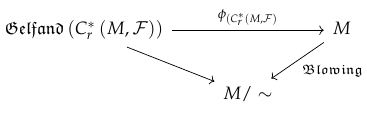
\includegraphics[width=0.5\linewidth]{folidgm.png}
	%		\caption{A boat.}
	%		\label{fig:boat1}
\end{figure}
\end{frame}
\begin{frame}
Roughly speaking the quotient is a map from Hausdorff blowing-up $M$ to the spectrum $M/\sim$. Hausdorff blowing-up is inverse operation. The following picture illustrates this statement
	\begin{figure}
	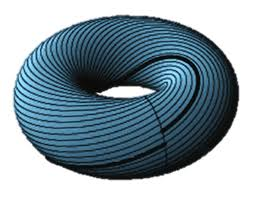
\includegraphics[width=0.5\linewidth]{nt.png}
	%		\caption{A boat.}
	%		\label{fig:boat1}
\end{figure}

\end{frame}
\section{Connes quantization}
\begin{frame}
	In general the quantization yields a passage from the classical physics to the quantum one. In particular there is a quantization which yields an the transformation from commutative $C^*$-algebra $B$ to noncommutative one. In particular a commutative  $C^*$-algebra $B$ with the product $\times$ is a depending on real parameter $\hslash$  limit of continuous fields  of noncommutative $C^*$-algebras $\overline B_\hslash$ with product $\times_\hslash$ such that
	\begin{itemize}
		\item Any $\overline B_\hslash$ is isomorphic to $B$ with the $C^*$-norm $f \mapsto \left\|f \right\|_{\hslash}$ which is continuous of $\hslash$ for any $f \in B$. 
		\item For any $f, g \in B$ we have $\left\|\left(f\times_\hslash g - g\times_\hslash f \right) /\hslash - i\left\{f, g\right\} \right\|_{\hslash}$ as $\hslash\to 0$, where $\left\{ ,\right\}_J$ is the Poisson bracket'
	\end{itemize}
\end{frame}
\section{Connes quantization}
\begin{frame}
 Hausdorff blowing-up equation
\be\label{blowing_r_eqn}
\mathfrak {Blowing}_{\sX-A }:C_0\left( \sX\right) \hookto M\left(A \right)
\ee
contains both a commutative $C^*$-algebra $C_0\left( \sX\right)$ and  a noncommutative one $A$. Elements of  $C_0\left( \sX\right)$  are limits of elements of $A$ with respect to the strict topology of $M\left(A \right)$, i.e. one has passage form noncommutative $C^*$-algebra to commutative one.



 This duality can have rich structure. It is known the physical fields (e.g. electromagnetic, electroweak etc.) correspond to vector bundles, or equivalently projective modules. We have constructed is  a bridge between projective $C\left(\sX^+ \right)$-modules and  $A^+$-modules. Physically it means that there is a set of classical projective modules  are common fields belonging to classical geometry and noncommutative one. The Rieffel projection on the noncommutative torus  correspond to a quantum projective module. This circumstance can have following physical interpretation. Classical fields correspond  to the "experimentally  proven" phenomena.  
\end{frame}
\begin{frame}
Rieffel projection is responsible for phenomena which cannot be easily detected, e.g. vanishing of the divergences.  	This analogy can be extended. For example the Dirac operator of noncommutative torus coincides with commutative one.
Sometimes this duality comes from the given by Alain Connes  algebraic counterpart of geometric quotient  which makes a non Hausdorff spectrum from a Hausdorff space. In this case we say that there is  \alert{ Connes quantization}.

	\end{frame}

\begin{frame}
	\alert{Thank you}
\end{frame}

\end{document}























